\documentclass{beamer}
%
% Choose how your presentation looks.
%
% For more themes, color themes and font themes, see:
% http://deic.uab.es/~iblanes/beamer_gallery/index_by_theme.html
%
%\input{header-pke.tex}

\mode<presentation>
{
  \usetheme{Darmstadt}      % or try Darmstadt, Madrid, Warsaw, ...
  \usecolortheme{default} % or try albatross, beaver, crane, ...
  \usefonttheme{default}  % or try serif, structurebold, ...
  \setbeamertemplate{navigation symbols}{}
  \setbeamertemplate{caption}[numbered]
} 

\usepackage[english]{babel}
\usepackage[utf8x]{inputenc}
\usepackage{fourier,eucal}
\usepackage{amsmath,amsfonts,amssymb}
\usepackage{color,multirow,dashbox}
\usepackage[]{algorithm2e}




\title[Your Short Title]{2-24-1 Optimization and search heuristics}
\author{Baptiste Louf, Yann Ramusat}
%%\institute{Ecole Polytechnique (intern at ENS Paris)}
\date{February $21^{st}$, 2017}

\begin{document}

\begin{frame}
  \titlepage
\end{frame}


\begin{frame}{Outline of the algorithm}
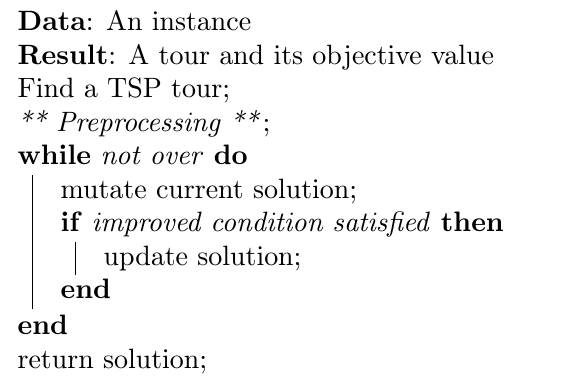
\includegraphics[scale=0.5]{algo}
\end{frame}

\begin{frame}{Choices made}
\begin{itemize}
\item Finding the tour
\begin{itemize}
\item TSP tour, otherwise too complicated
\item Nice research question : define a good tour for the TTP and compute it
\end{itemize}
\item Preprocessing
\begin{itemize}
\item Remove "disadvatadgeous items"
\item No improvement, overfitting
\end{itemize}
\end{itemize}

\end{frame}



\begin{frame}{Heuristics}
\begin{itemize}
\item RLS
\item ($\mu$+$\lambda$) EA
\begin{itemize}
\item $\mu=1$, $\lambda=7$
\end{itemize}
\item Simulated annealing
\begin{itemize}
\item probability of "going backwards" $=e^{-d\log(n)/100}$
\end{itemize}
\item ($\mu$,$\lambda$) EA
\begin{itemize}
\item $\mu=1$, $\lambda=7$
\end{itemize}
\item 1+($\lambda$,$\lambda$) GA
\item Random mutation
\begin{itemize}
\item RLS mutation w.p. $1/2$, ($\mu$+$\lambda$) mutation w.p. $1/2$
\end{itemize}
\end{itemize}


\end{frame}
\begin{frame}{Methodology}
\begin{itemize}
\item datasets of the CEC competition
\item time limit of 10 minutes
\item stops if 1000000 steps without improvement
\item 3 runs of each algorithm
\end{itemize}

\end{frame}

\begin{frame}{Results}
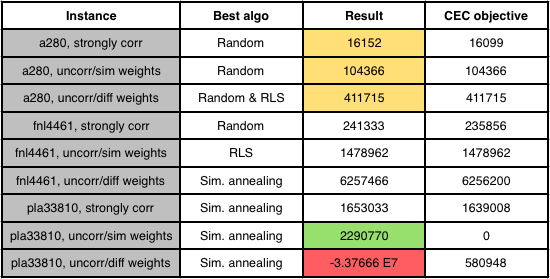
\includegraphics[scale=0.6]{tableau}
\end{frame}

\end{document}